\documentclass[a4paper,11pt]{article}
\usepackage[utf8]{inputenc}
\usepackage[T1]{fontenc}
\usepackage[english]{babel}
\usepackage{amsmath,amssymb,amsthm,amsfonts}
\usepackage{graphicx}

\title{
	Computer Exercise 3\\
	EL2520 Control Theory and Practice
}
\author{
	Jean-Alix David\\
	jadavid@kth.se\\
	90061T314
	\and
	Kilian Demeulemeester\\
	kiliande@kth.se\\
	910308T213
}

\begin{document}
	\maketitle

	% Suppression of outputs
	\section*{Suppression of outputs}

	The weight is
	\begin{align*}
        W_S(s) = \frac{10^{4}}{(s+p_1)(s+p_2)} 
	\end{align*}
    With $p_{1,2} = -.1 \pm \sqrt{(100\pi)^2-.1^2}$ 
    % -1e-3 + 3.14e2i and conjugate
    % P = 1e4

    \begin{figure}[h!b]
        \centering
        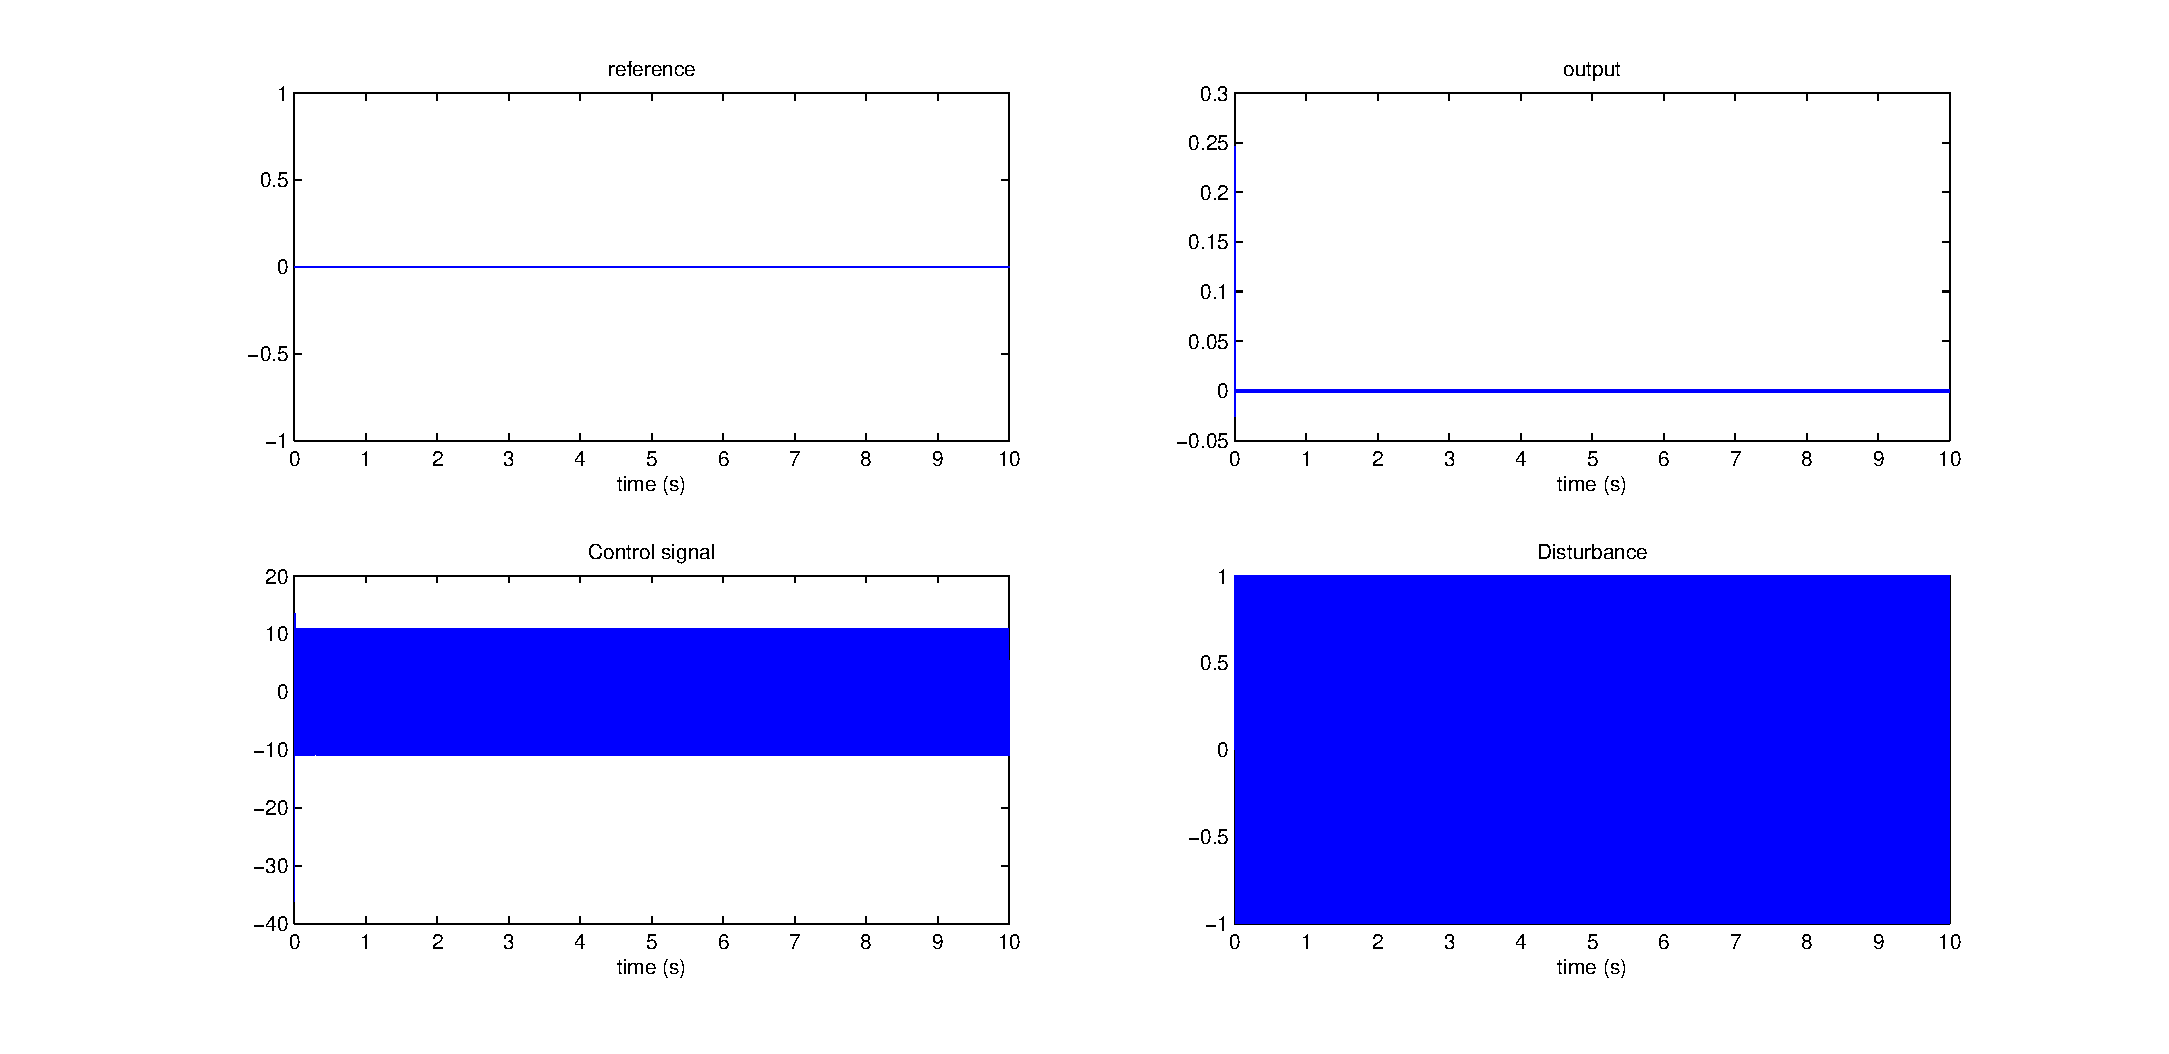
\includegraphics[width=.75\columnwidth]{fig/figure1.eps}
        \caption{Simulation results}
    \end{figure}

    The simulation results are the following:
    \begin{center}
        \begin{tabular}{|c|c|}
        \hline
        \textbf{Signal} & \textbf{Amplitude} \\
        \hline
        output ($y$) & $10^{-4}$ \\
        \hline
        control signal ($u$) & $\approx 10$ \\
        \hline
        \end{tabular}
    \end{center}

    Using a P-controller with $P(s) = 10^6$ leads to the same performance results. 
    However such a controller gives less flexibility towards the frequence rejection (all frequency will have the same amplification / atenuation).

	% Robustness
	\section*{Robustness}

    The small gain theroem relation is:
    \begin{align*}
        |T(i\omega)| < \frac{1}{|\Delta_G(i\omega)|}
    \end{align*}
    Here:
    \begin{align*}
        \frac{1}{\Delta_G(i\omega)} = \frac{|s+2|}{3}
    \end{align*}

	Therefore the weights are
	\begin{align*}
        W_S(s) & = \frac{10^{4}}{(s+p_1)(s+p_2)}  \\
        W_T(s) & = \frac{3}{s+2}
	\end{align*}

	% \image{fig/figure2.eps}{Simulation results}
    \begin{figure}[h!b]
        \centering
        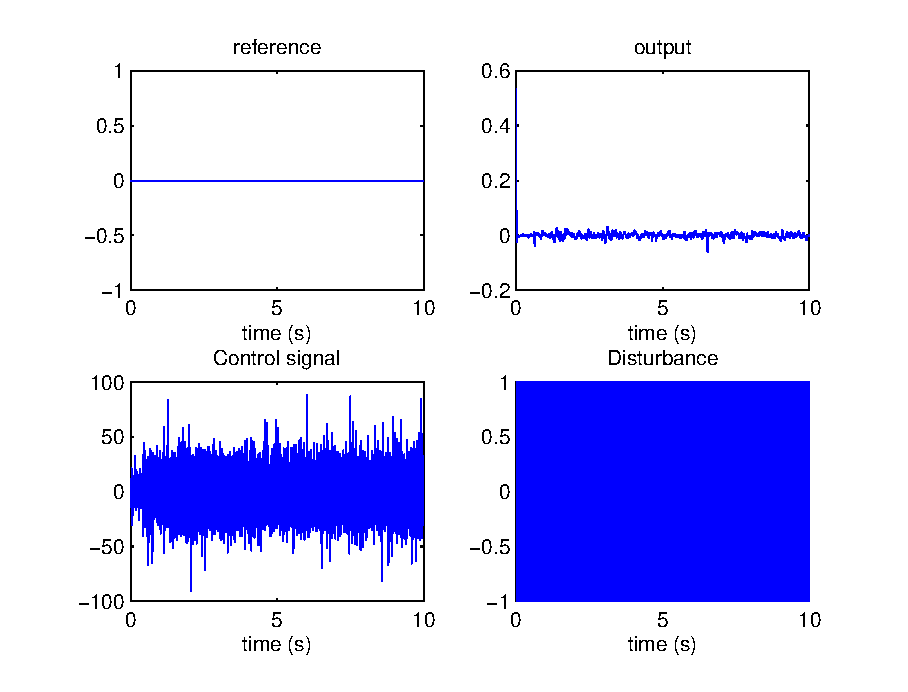
\includegraphics[width=.75\columnwidth]{fig/figure2.eps}
        \caption{Simulation results}
    \end{figure}

    The simulation result using $G_0$ are:
    
    \begin{center}
        \begin{tabular}{|c|c|}
        \hline
        \textbf{Signal} & \textbf{Amplitude} \\
        \hline
        output ($y$) & $10^{-2}$ \\
        \hline
        control signal ($u$) & $\approx 50$ \\
        \hline
        \end{tabular}
    \end{center}

	\section*{Control signal}

    Here the weight are:
	
    \begin{align*}
        W_S(s) &= \frac{10^{4}}{(s+p_1)(s+p_2)}  \\
        W_T(s) &= \frac{3}{s+2} \\
        W_U(s) &= \frac{10^{2}}{(s+p_1)(s+p_2)}  
	\end{align*}

    \begin{figure}[h!b]
        \centering
        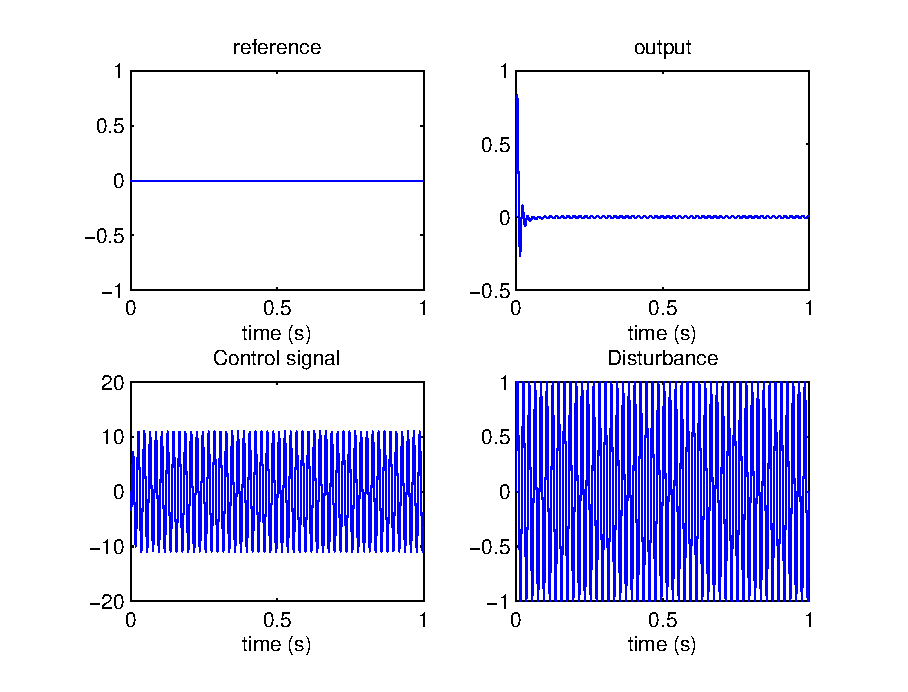
\includegraphics[width=.75\columnwidth]{fig/figure3.eps}
        \caption{Simulation results}
    \end{figure}

    The simulation result with all of the controls are:
    \begin{center}
        \begin{tabular}{|c|c|}
        \hline
        \textbf{Signal} & \textbf{Amplitude} \\
        \hline
        output ($y$) & $10^{-3}$ \\
        \hline
        control signal ($u$) & $\approx 10$ \\
        \hline
        \end{tabular}
    \end{center}

    We have decrease the control signal amplitude to one fifth of the previous values. The output amplitude has also decrease. 



\end{document}
